\section{Generalities}

To run a \MMonCa\ script just call the {\param mmonca} binary with the input file you want to execute as a parameter name.

\begin{lstlisting}
mmonca input.mc
\end{lstlisting}

The input scripts are regular \param{TCL} scripts that include additional MMonCa commands. All regular TCL commands (to manipulate variables, loops, procedures, etc) should be available. For a list of the additional commands included in \MMonCa\ allowing Monte Carlo simulations and post-processing of information, consult Chapter~\ref{chap:commands}.

\subsection{Starting from scratch}

The following is a list of required and optional instructions that should be provided in a \MMonCa\ script when starting from scracth:

\begin{description}
\item [required] Telling MMonCa with materials to use by setting {\param MC/General/materials}
\item [required] Defining the distribution of materials in space with a procedure ({\tt proc material} in this case)
\item [optional] Redefining some extra parameters with \param{param}.
\item [required] Initializing the simulation box with \param{init}.
\item [optional] Reading the initial damage to anneal with \param{cascade}.
\item [required] Letting the system evolve in time with the \param{anneal}.
\item [optional] Obtaining some useful information with \param{extract}.
\item [optional] Saving some information for visualization purposes with \param{save}.
\item [optional] Saving the simulation status for restarting with \param{restart}.
\end{description}

\subsection{Restarting}

An alternative is to start \MMonCa\ from a file saved with the \param{restart} option. In this case, the following is the list of required and optional instructions:
\begin{description}
\item [required] Using the \param{restart} option as the first command.
\item [optional] Redefining some extra parameters with \param{param}.
\item [optional] Reading the initial damage to anneal with \param{cascade}.
\item [optional] Letting the system evolve in time with the \param{anneal}.
\item [optional] Obtaining some useful information with \param{extract}.
\item [optional] Saving some information for visualization purposes with \param{save}.
\item [optional] Saving the simulation status for further restarting with \param{restart}.
\end{description}


\section{Object Kinetic Monte Carlo simulation: an example}

The following is an example of a \MMonCa\ input script, taken from Ref.~\cite{MARTIN-BRAGADO-CPC13}, that performs the isochronal annealing of $\alpha$-Fe. The goal is to simulate the evolution of defects and resistivity recovery during isochronal annealing of high-purity electron-irradiated iron. The script contains both the commands needed to set the simulation conditions, and the commands required to do some post-processing of information, mainly extracting the evolution of defects with time to an external file. There are also typical \param{TCL} commands that help in the extraction. 

The initial damage in this example is read from an {\tt electron.cascade} file containing the IV pairs produced by electron irradiation.

This example can be found in the {\param examples} directory.

\subsection{The script}

\begin{lstlisting}
param set type=map<string,string>   key=MC/General/materials value="S_Iron Fe"
set size 143.5
set time 300

proc material { x y z } { return "S_Iron" }

#parameters
param set type=bool   key=MC/Mesh/periodic.x value=true

param set type=arrhenius key=S_Iron/Vacancy/V(migration)   value="5e-5 0.67"
param set type=arrhenius key=S_Iron/Iron/I(migration)      value="3.2e-3 0.34"

init minx=0 miny=0 minz=0 maxx=$size maxy=$size maxz=$size material=material

cascade file=electron.cascade format=B:C*.287:D*.287:E*.287 periodic flux=4.8562e9 do.not.react

set X 0
set a 77.2
set b 1.030927

set FILE [open "results.txt" w]
close $FILE

set oldTotal 0
set oldC 0

save ovito=evolution
while { $X < 65 } {
      incr X
      set c [expr $a*$b]
      lowmsg "Running for $c K"      
      set FILE [open "results.txt" a]
      anneal time=$time temp=[expr $c - 273.15]
      save ovito=evolution append
      set total [extract count.particles]
      set deriv [expr ($total - $oldTotal)/($c - $oldC)]
      set I     [extract count.particles particle=I defect=MobileParticle]
      set V     [extract count.particles particle=V defect=MobileParticle]
      set I2    [extract count.particles defect=ICluster ID=I2]
      set V2    [extract count.particles defect=VCluster ID=V2]
      set I3    [extract count.particles defect=ICluster ID=I3]
      set V3    [extract count.particles defect=VCluster ID=V3]
      set I111  [extract count.particles defect=<111>]
      set oI    [expr [extract count.particles defect=ICluster] -$I2 -$I3]
      set oV    [expr [extract count.particles defect=VCluster] -$V2 -$V3]
      puts $FILE "$c $total $deriv $I $V $I2 $V2 $I3 $V3 $oI $oV $I111"
      lowmsg     "$c $total $deriv $I $V $I2 $V2 $I3 $V3 $oI $oV $I111"
      close $FILE
      set a $c
      set oldC $c
      set oldTotal $total
}
\end{lstlisting}

\subsection{The script, dissected}

\begin{lstlisting}
param set type=map<string,string>   key=MC/General/materials value="S_Iron Fe"
\end{lstlisting}
Line needed to define the materials to be used in the simulation.

\begin{lstlisting}[firstnumber=2]
set size 143.5
set time 300
\end{lstlisting}
TCL variables defined to easily change the simulation size and the annealing times between steps.

\begin{lstlisting}[firstnumber=5]
proc material { x y z } { return "S_Iron" }
\end{lstlisting}
Required script to define the material in the simulation. In this case, a block containing only Iron is defined.

\begin{lstlisting}[firstnumber=7]
#parameters
param set type=bool   key=MC/Mesh/periodic.x value=true
param set type=arrhenius key=S_Iron/Vacancy/V(migration)   value="5e-5 0.67"
param set type=arrhenius key=S_Iron/Iron/I(migration)      value="3.2e-3 0.34"
\end{lstlisting}
Some redefinition of parameters: setting of periodic boundary conditions in x (false by default, because there are usually free surfaces in this axis), and small changes in point defect migration parameters.

\begin{lstlisting}[firstnumber=13]
init minx=0 miny=0 minz=0 maxx=$size maxy=$size maxz=$size material=material
\end{lstlisting}
Required initialization of the simulator, specifying the simulation sizes and the script containing the material definition. In this case, we are using the TCL variables, previously defined, {\tt size}.

\begin{lstlisting}[firstnumber=15]
cascade file=electron.cascade format=B:C*.287:D*.287:E*.287 periodic flux=4.8562e9 do.not.react
\end{lstlisting}
Initial conditions for the simulation: insertion of damage. This command is not strictly needed, but is very common, because damage has to be introduced to simulate its evolution, unless equilibrium concentrations want to be set.

\begin{lstlisting}[firstnumber=17]
set X 0
set a 77.2
set b 1.030927
\end{lstlisting}
Definition of some convenient TCL variables to later compute the temperature ramps.

\begin{lstlisting}[firstnumber=21]
set FILE [open "results.txt" w]
close $FILE
\end{lstlisting}
This confusing commands open a file to close it right away. The goal is to overwrite previous existing files with an empty file. Later, information will be appended to the file.

\begin{lstlisting}[firstnumber=24]
set oldTotal 0
set oldC 0
\end{lstlisting}
Definition of TCL variables to compute the first derivative of the total damage.

\begin{lstlisting}[firstnumber=27]
save lammps=evolution
\end{lstlisting}
Command to create a initial file with the atomistic information, using the \param{lammps} format that can be later used by \param{ovito} to visualize the information. More save commands will be issued later to \param{append} new time frames into the file.

\begin{lstlisting}[firstnumber=28]
while { $X < 65 } {
      incr X
      set c [expr $a*$b]
      lowmsg "Running for $c K"      
\end{lstlisting}
Initialization of the loop to increase the temperature, and operations to compute the next temperature for the annealing.

\begin{lstlisting}[firstnumber=32]
      set FILE [open "results.txt" a]
\end{lstlisting}
TCL command to open an (existing) file and append information to it.

\begin{lstlisting}[firstnumber=33]
      anneal time=$time temp=[expr $c - 273.15]
\end{lstlisting}
The fundamental \param{anneal} command, needed to start the annealing of defects in time. Both the time and temperature need to be specified, in this case, using TCL variables defined previously. Since the temperature in ``c'' is in Kelvin, but the anneal command requires the temperature to be written in Celsius, a translation is defined in line.

\begin{lstlisting}[firstnumber=34]
      save lammps=evolution append
\end{lstlisting}
Command to append one more snapshot for visualization

\begin{lstlisting}[firstnumber=35]
      set total [extract count.particles]
      set deriv [expr ($total - $oldTotal)/($c - $oldC)]
      set I     [extract count.particles particle=I defect=MobileParticle]
      set V     [extract count.particles particle=V defect=MobileParticle]
      set I2    [extract count.particles defect=ICluster ID=I2]
      set V2    [extract count.particles defect=VCluster ID=V2]
      set I3    [extract count.particles defect=ICluster ID=I3]
      set V3    [extract count.particles defect=VCluster ID=V3]
      set I111  [extract count.particles defect=<111>]
      set oI    [expr [extract count.particles defect=ICluster] -$I2 -$I3]
      set oV    [expr [extract count.particles defect=VCluster] -$V2 -$V3]
      puts $FILE "$c $total $deriv $I $V $I2 $V2 $I3 $V3 $oI $oV $I111"
      lowmsg     "$c $total $deriv $I $V $I2 $V2 $I3 $V3 $oI $oV $I111"
      close $FILE
\end{lstlisting}
Post-processing of the information after each annealing. The number of particles for different defect types is asked, and stored in TCL variables.  These variables are used to add one line to the previously opened file, with the different values, then allowing to have a file with different columns, and the number of particles of different defects in each column. The derivative of the number of defects is also computed.

\begin{lstlisting}[firstnumber=49]
      set a $c
      set oldC $c
      set oldTotal $total
}
\end{lstlisting}
Variable operations to update the temperature ramp, and to make possible the computation of the first derivative. End of the script.

\subsection{The output}

The script creates a list named {\tt results.txt} that looks like:
\begin{verbatim}
79.58756439999999 59955 753.3212060450993 29962 29993 0 0 0 0 0 0 0
82.04896900419878 59955 0.0 29962 29993 0 0 0 0 0 0 0
84.58649746859163 59953 -0.7881684986255068 29961 29992 0 0 0 0 0 0 0
87.20250407580276 59937 -6.116192503449846 29953 29984 0 0 0 0 0 0 0
89.8994159193551 59917 -7.415889417303392 29943 29974 0 0 0 0 0 0 0
92.67973515549299 59813 -37.40577651955731 29891 29922 0 0 0 0 0 0 0
95.54604132464692 59453 -125.59718981669849 29711 29742 0 0 0 0 0 0 0
98.50099374469427 58089 -461.5979569573388 29029 29060 0 0 0 0 0 0 0
101.54733397823642 54015 -1337.342413412217 26978 27023 14 0 0 0 0 0 0
104.68788837618133 43219 -3437.6096166538605 21560 21625 34 0 0 0 0 0 0
107.92557069999148 23693 -6030.857276022542 11749 11862 82 0 0 0 0 0 0
111.26338482503012 9445 -4268.661904543617 4601 4738 106 0 0 0 0 0 0
114.70442752751381 6359 -896.8211867212708 3060 3195 104 0 0 0 0 0 0
118.25189135765723 5303 -297.6774536859221 2516 2667 120 0 0 0 0 0 0
121.90906760167549 4757 -149.2955120478667 2229 2394 134 0 0 0 0 0 0
125.6793493353925 4399 -94.95311631448243 2015 2215 166 0 3 0 0 0 0
129.56623457228818 4087 -80.26992848628163 1811 2059 214 0 3 0 0 0 0
133.57332950890532 3801 -71.3734025581751 1493 1916 374 0 18 0 0 0 0
137.70435187062722 3439 -87.62963942153782 1100 1735 500 0 96 0 8 0 0
141.9631343609301 2967 -110.82979726593929 611 1499 604 0 213 0 40 0 0
146.3536282173106 2535 -98.39439801793499 229 1283 604 0 303 0 108 0 8
150.87990687718735 2327 -45.9538653339702 44 1179 578 0 327 0 184 0 15
\end{verbatim}

\begin{figure}
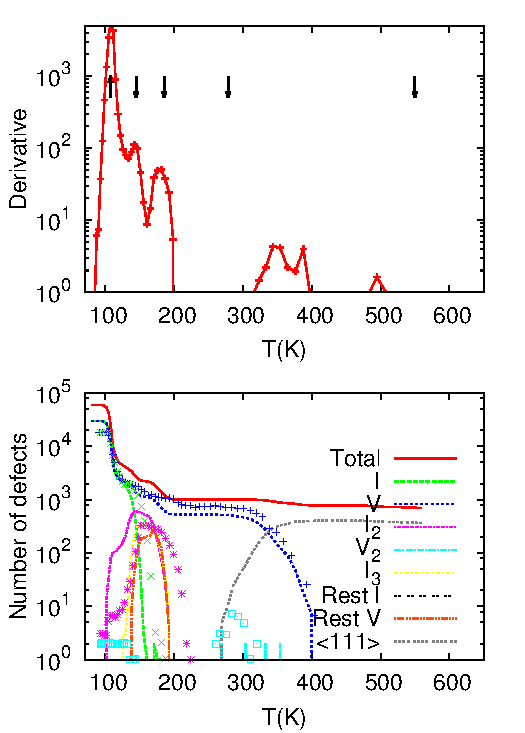
\includegraphics{images/Fe}
\caption{Isochronal annealing of Iron. \cite{MARTIN-BRAGADO-CPC13}}
\label{fig:isochronalFe}
\end{figure}


Fig.~\ref{fig:isochronalFe} shows the results processed with the \param{gnuplot} tool.



\section{Lattice Kinetic Monte Carlo simulation: an example}

In this section we will show an input script that, using the Lattice Kinetic Monte Carlo model, simulates the Si(100), Si(011) and Si(111) Solid Phase epitaxial regrowth of a partially amorphized sample, and computes its recrystallization speed and roughness. These scripts used the models published in Refs.~\cite{MARTIN-BRAGADO-APL09,MARTIN-BRAGADO-APL11,MARTIN-BRAGADO-SM12,MARTIN-BRAGADO-JAP12}, and are partially based in the scripts distributed under the folder \param{tests}, sub-folders {\tt standard/lkmc}.

\subsection{The script}

\begin{lstlisting}
param set type=map<string,string>   key=MC/General/materials value="Silicon Si AmorphousSilicon aSi Gas Gas"

set T 550
set name SPER
#0 9 or 14
set i 0
proc material { x y z } {
        set res "Unknown"
        if { $x < 0 } {
                set res "Gas"
        } elseif { $x < 52 } {
                set res "AmorphousSilicon"
        } else {
                set res "Silicon"
        }
        return $res
}

set angle(0)  00
set angle(9)  55
set angle(14) 90

set sizeZ    [expr sqrt(2.)*.5431*26]
set sizeY    [expr 180]

param set type=bool key=MC/Mesh/periodic.y value=false
param set type=bool key=MC/Mesh/periodic.z value=true

set radians "$angle($i).0*2.0*3.1415926535897931/360.0"
set S [expr sin($radians)]
set C [expr cos($radians)]
set R [expr sqrt(2.0)]
set waferorient "i $C  j [expr $S/$R] k [expr $S/$R]"
set flatorient  "i -$S j [expr $C/$R] k [expr $C/$R]"

param set type=map<string,float> key=Silicon/Lattice/wafer.orientation value="$waferorient"
param set type=map<string,float> key=Silicon/Lattice/flat.orientation  value="$flatorient" 
param set type=map<string,float> key=AmorphousSilicon/Lattice/wafer.orientation value="$waferorient"
param set type=map<string,float> key=AmorphousSilicon/Lattice/flat.orientation  value="$flatorient" 

init minx=-2 miny=0 minz=0 maxx=54 maxy=$sizeY maxz=$sizeZ material=material

anneal time=1 temp=$T depth=51
set orig_time [extract time]  
set orig_depth [lindex [extract ac.mean min.y=60 max.y=120 min.z=0 max.z=$sizeZ] 0]
lowmsg "Original depth is $orig_depth"

anneal time=1 temp=$T depth=31
set end_time [extract time]   
set end_depth [lindex [extract ac.mean min.y=60 max.y=120 min.z=0 max.z=$sizeZ] 0]
lowmsg "$angle($i) - Final depth is $end_depth"
set velocity [expr ($orig_depth - $end_depth)/($end_time-$orig_time)*60]
set roughnes [extract ac.stdev]
lowmsg "Velocity  for angle $angle($i) is $velocity in nm/min."
lowmsg "Roughness for angle $angle($i) is $roughnes in nm."

\end{lstlisting}

\subsection{The script, dissected}

This script adds the complication that it has been done to accept different substrate orientation with minimum changes in the script. This complication is managed using a TCL array called {\tt angle}, and used to compute the substrate orientation automatically. Also, since having periodic boundary conditions is not possible for all possible substrate orientations, the script defines a quite large $y$ domain (180\,nm) without boundary conditions, but measures the recrystallization velocity only in the middle of the domain, where it is expected to be flat.

\begin{lstlisting}
param set type=map<string,string>   key=MC/General/materials value="Silicon Si AmorphousSilicon aSi Gas Gas"
\end{lstlisting}
Definition of the materials used.

\begin{lstlisting}[firstnumber=3]
set T 550
set name SPER
\end{lstlisting}
Definition of temperature and script name, to be used later

\begin{lstlisting}[firstnumber=5]
#0 9 or 14
set i 0
\end{lstlisting}
The substrate angle is codified in this integer.

\begin{lstlisting}[firstnumber=7]
proc material { x y z } {
        if { $x < 0 } {
                set res "Gas"
        } elseif { $x < 52 } {
                set res "AmorphousSilicon"
        } else {
                set res "Silicon"
        }
        return $res
}
\end{lstlisting}
Definition of the materials. Three sections are defined, ``Gas'', for $x < 0$, ``AmorphousSilicon'' for $0 < x < 52$ and ``Silicon'' (i.e., crystalline silicon) for $x \geq 52$.

\begin{lstlisting}[firstnumber=19]
set angle(0)  00
set angle(9)  55
set angle(14) 90
\end{lstlisting}
Definition of an array indexed by integers with the possible angles. 0 for Si(100), 9 for Si(111) and 14 for Si(011). This infrastructure allows the definition of intermediate angles for the other $i$s.

\begin{lstlisting}[firstnumber=23]
set sizeZ    [expr sqrt(2.)*.5431*26]
set sizeY    [expr 180]
\end{lstlisting}
Definition of the size as a variable. $y$ should be big enough to have a flat region without periodic boundary conditions, but especial dimensions are set for $z$ to have periodicity.

\begin{lstlisting}[firstnumber=26]
param set type=bool key=MC/Mesh/periodic.y value=false
param set type=bool key=MC/Mesh/periodic.z value=true
\end{lstlisting}
Boundary conditions for $z$ only. By default $x$ has no PBC.

\begin{lstlisting}[firstnumber=29]
set radians "$angle($i).0*2.0*3.1415926535897931/360.0"
set S [expr sin($radians)]
set C [expr cos($radians)]
set R [expr sqrt(2.0)]
set waferorient "i $C  j [expr $S/$R] k [expr $S/$R]"
set flatorient  "i -$S j [expr $C/$R] k [expr $C/$R]"
\end{lstlisting}
Example of use of the TCL language embedded in the \MMonCa\ scripting to compute the substrate orientation.

\begin{lstlisting}[firstnumber=36]
param set type=map<string,float> key=Silicon/Lattice/wafer.orientation value="$waferorient"
param set type=map<string,float> key=Silicon/Lattice/flat.orientation  value="$flatorient" 
param set type=map<string,float> key=AmorphousSilicon/Lattice/wafer.orientation value="$waferorient"
param set type=map<string,float> key=AmorphousSilicon/Lattice/flat.orientation  value="$flatorient" 
\end{lstlisting}
Definition of the substrate orientation as a parameter, once computed previously.

\begin{lstlisting}[firstnumber=41]
init minx=-2 miny=0 minz=0 maxx=54 maxy=$sizeY maxz=$sizeZ material=material
\end{lstlisting}
Compulsory definition of the initial simulation box and initial materials.

\begin{lstlisting}[firstnumber=43]
anneal time=1 temp=$T depth=51
\end{lstlisting}
Since the amorphous/crystalline (A/C) interface is artificially flat plane (atomically flat) an small initial annealing (recrystallization) is issued to recrystallize a maximum of 1\,nm, creating an starting condition where the A/C interface is more realistic. 

\begin{lstlisting}[firstnumber=44]
set orig_time [extract time]  
set orig_depth [lindex [extract ac.mean min.y=60 max.y=120 min.z=0 max.z=$sizeZ] 0]
lowmsg "Original depth is $orig_depth"
\end{lstlisting}
Use of TCL to store the initial position of the interface.

\begin{lstlisting}[firstnumber=48]
anneal time=1 temp=$T depth=31
\end{lstlisting}
Main recrystallization: From depth 51 to depth 31, a maximum of 20\,nm is requested.

\begin{lstlisting}[firstnumber=49]
set end_time [extract time]   
set end_depth [lindex [extract ac.mean min.y=60 max.y=120 min.z=0 max.z=$sizeZ] 0]
lowmsg "$angle($i) - Final depth is $end_depth"
set velocity [expr ($orig_depth - $end_depth)/($end_time-$orig_time)*60]
set roughnes [extract ac.stdev]
\end{lstlisting}
The annealing command stops when the A/C touches the requested depth, but here we want to compute the recrystallization speed using average values, not maximum ones. Thus, the average depth is computed for $60 < y < 120$ and stored. The velocity is then computed using the regular $v=\frac{\Delta x}{\Delta t}$ equation. The roughness is extracted using a specific \MMonCa\ command.

\begin{lstlisting}[firstnumber=54]
lowmsg "Velocity  for angle $angle($i) is $velocity in nm/min."
lowmsg "Roughness for angle $angle($i) is $roughnes in nm."
\end{lstlisting}
Finally, the values are displayed.

\subsection{Simulation results}

Fig.~\ref{fig:lkmc-example} shows the results for Si(100), Si(011) and Si(111) simulations compared to experimental results taken from Ref.~\cite{CSEPREGI-JAP78}

\begin{figure}
\begin{center}
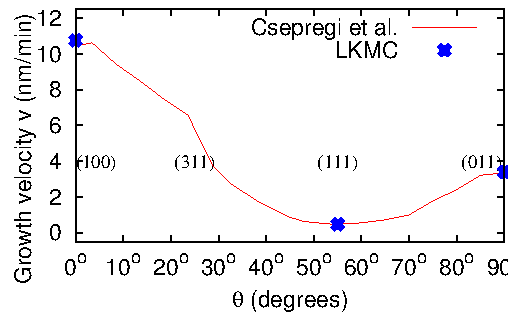
\includegraphics{images/csepregi}
\end{center}
\caption{Solid Phase Epitaxial Regrowth of amorphized silicon. \cite{MARTIN-BRAGADO-APL09}}
\label{fig:lkmc-example}
\end{figure}
